\section{Physical Simulation}

\begin{figure}[h]
  \centering
  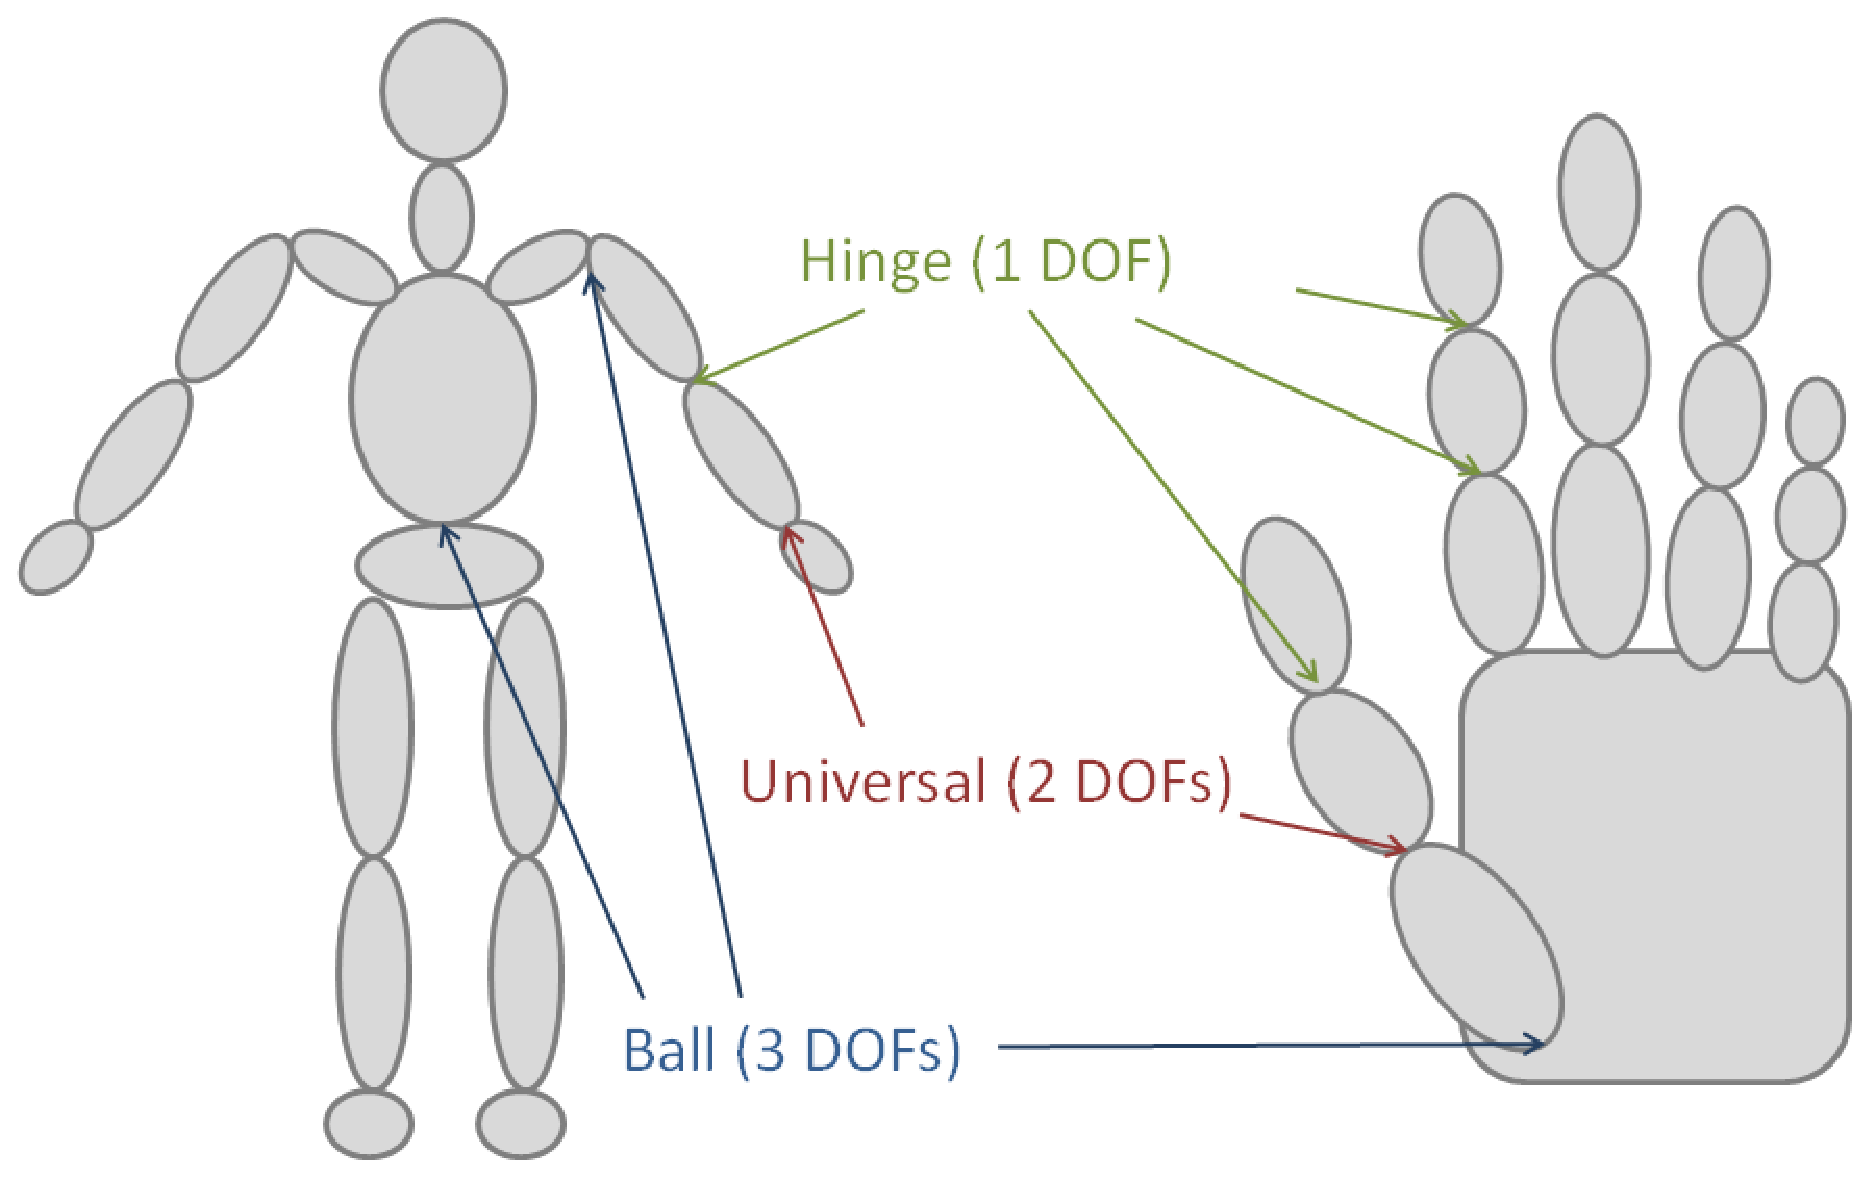
\includegraphics[width=0.6\textwidth]{figures/character}
  \caption{Articulated figures in character animation to represent a human character (left) and a hand (right).}
  \label{fig:character}
\end{figure}


In most of physically-based character animation systems, human characters are represented as an articulated rigid body system (Figure \ref{fig:character} left), a group of rigid bodies chained together through rotational joints. These joints can have different number of degrees of freedom (DOF). For example, the shoulder is a ball joint with three DOFs. The wrist is an universal joint (2 DOFs) and the elbow is a hinge joint (1 DOF). In some cases, if the character's motion involves dexterous hand manipulation, a more detailed hand model (Figure \ref{fig:character} right) is attached to the wrist. Note that this human model is a drastic simplification since simulating each bone, muscle and tendon that a real human has would require a prohibitively huge amount of computational resources. The articulated figure is represented as a tree structure. Each node is a rigid body and each edge is a joint. Each node can have multiple children but at most one parent. The root node has no parent. Note that in this tree representation, loop is not allowed. Although it is possible to simulate loops, such case is rare in character animation and will not discussed here. There are two major methods to simulate the dynamics of an articulated rigid body system. It can be simulated in maximal coordinates (Cartesian space) or in generalized coordinates (joint space).



\subsection{Simulation in maximal coordinates}

In maximal coordinates, the physical states of the articulated figures are defined for each node (rigid body). Each body has six degrees of freedom: three translational and three rotational. The dynamics of each rigid body is considered independently. A list of additional joint constraints are imposed to ensure that the two adjacent bodies will stick together at the joint location. The dynamics equation for each body is 

\begin{equation}
\left[\begin{array}{cc}
m\vc{I}_{3\times3} & \vc{0} \\
\vc{0} & \vc{I}
\end{array}\right]
\left[\begin{array}{c}
\dot{\vc{v}} \\
\dot{\vc{\omega}}
\end{array}\right]=
\left[\begin{array}{c}
m\vc{g} \\
-\dot{\vc{I}}\vc{\omega}
\end{array}\right]
+\left[\begin{array}{c}
\vc{I}_{3\times3}\\
\vc{[r]}_\times
\end{array}\right]
\vc{f}+
\left[\begin{array}{c}
\vc{0}\\
\boldsymbol{\tau}_c+\boldsymbol{\tau}
\end{array}\right]
\label{eq:dynamics}
\end{equation}
where $m$ and $\vc{I}$ are the mass and the inertia tensor of the body. $\vc{I}_{3\times 3}$ is a $3\times 3$ identity matrix. $\vc{v}$ and $\vc{\omega}$ are the linear and angular velocities. $\vc{f}$ consists of joint constraint forces and contact forces. $\vc{r}$ is the vector from the center of mass to the point that $\vc{f}$ acts upon. $[\vc{r}]_{\times}$ is the skew symmetric matrix that maps $\vc{f}$ to its corresponding torque. $\boldsymbol{\tau}_c$ is the joint constraint torque while $\boldsymbol{\tau}$ is the torque exerted by the actuators.

Joints that connect two rigid bodies constrain their relative motions. Different number of constraints are imposed according to the type of joints. For example, a fix joint has six constraints, which entirely eliminate the relative motion between two two adjacent bodies. A hinge joint has five constraints that eliminate all but the rotation along the joint axis. A ball joint has three, which only constrains the relative translation at the joint location. 

Suppose a joint connects body $A$ and body $B$, each constraint is a linear equality:

\begin{equation}
\vc{J}_A
\left[\begin{array}{c}
\vc{v}_A \\
\vc{\omega}_A
\end{array}\right]-
\vc{J}_B
\left[\begin{array}{c}
\vc{v}_B \\
\vc{\omega}_B
\end{array}\right]
=0
\label{eq:jointConstraint}
\end{equation}
where $\vc{J}_A$ is a row in the Jacobian matrix that maps the velocities of body $A$ to one component of the linear velocity at the joint position or the angular velocity perpendicular to the joint axes.

To allow a character to actively control its motion, actuators are attached to the joints. According to Newton's third law, the two bodies connected to a common actuator should receive equal and opposite joint torques.
\begin{equation}
\boldsymbol{\tau}_A-\boldsymbol{\tau}_B=0
\label{eq:actuatorConstraint}
\end{equation}
where $\boldsymbol{\tau}_A$ and $\boldsymbol{\tau}_B$ are the torques exerted by the actuator to body $A$ and $B$ respectively.

Although simple to understand and implement, simulating characters in maximal coordinates is not the most popular method due to a few drawbacks. First, the state representation in  maximal coordinates is redundant. It is not efficient to use all six degrees of freedom a rigid body and then eliminate most of them using joint constraints. Second, the accumulating numerical errors in simulation would cause the joint constraints not satisfied exactly. Eventually, joints will dislocate and adjacent bodies will drift apart. Both of these shorting comings are overcome by simulation in generalized coordinates.

\subsection{Simulation in generalized coordinates}
In generalized coordinates, the physical states $\vc{q}$ of the articulated figure are defined on the edges of the tree (joints). The root node is attached to the world space via a 6-dof free joint. It can translate and rotate freely. Other nodes can be attached to their parents through a 3-dof ball joint, 2-dof universal joint, 1-dof hinge joint or 0-dof fix joint. Each degree of freedom contributes one component of $\vc{q}$. The number of DOF's equals the dimensionality of $\vc{q}$. In other words, there is no redundancy in this representation.

The dynamics equation in generalized coordinates for an articulated rigid body system is:
\begin{equation}
  \vc{M}(\vc{q})\vc{\ddot{q}}+\vc{C(q,\dot{q})}=\vc{J}^T\vc{f}+\boldsymbol{\tau}
  \label{eq:generalized}
\end{equation}
where $\vc{q}$, $\vc{\dot{q}}$ and $\vc{\ddot{q}}$ are the position, velocity and acceleration in generalized coordinates. $\vc{M}$ is the mass matrix. $\vc{C(q,\dot{q})}$ accounts for the Coriolis and centrifual force. $\vc{J}$ is the Jacobian matrix. $\vc{f}$ is the external force in Cartesian space, such as gravity and contact force. $\boldsymbol{\tau}$ is the generalized force, including the actuator torques. This equation is derived from Lagrangian dynamics. Detailed derivation can be found in Liu and Jain \cite{Liu:2012:STM}.

When the articulated rigid bodies are simulated in generalized coordinates, it is often necessary to convert physical quantities back and forth between generalized and maximal coordinates. For example, we need to compute the velocity at certain point on the articulated figure in Cartesian space to collision detection. We also need to convert the forces from the Cartesian space to generalized coordinates to apply contact forces. The conversion is through the Jacobian matrix $\vc{J}$.
\begin{equation}
\vc{J}=\frac{\partial \vc{x}}{\partial \vc{q}}
\end{equation}
Jacobian matrix bridges the two different coordinate system. It represents the relation how much a point $\vc{x}$ moves in the Cartesian space if the joint angles $\vc{q}$ changes slightly. Here are two most frequently-used formulas that transfer velocities and forces:
\begin{displaymath}
  \begin{array}{lll}
    \vc{v} & = & \vc{J}\vc{\dot{q}}\\
    \boldsymbol{\tau} & = &\vc{J}^T\vc{f}
   \end{array}
\end{displaymath}
More conversion formulas can be found in Liu and Jain \cite{Liu:2012:STM}.

Simulation in generalized coordinates is commonly used in physically-based character animation. Although it takes more effort to walk through the derivation, it has important advantages over simulation in maximal coordinates. Apparently, the representation is more compact. There is no redundancy and thus no need to use constraints to eliminate redundant states. More importantly, this compactness ensures that the joints are preserved exactly: the two bodies that are chained together cannot drift apart due to accumulation of numerical errors. This is because state of dislocated bodies are not representable in generalized coordinates.

\subsection{Contact modeling}

Most tasks modeled in physically-based character animation, such as locomotion and hand manipulation, rely on accurately simulating the contacts between the human character and its physical environment. Penalty force and Linear Complementarity Problem (LCP) are two widely used methods in contact modeling.

\subsubsection{Penalty method}
When a body $A$ penetrates another body $B$, a repulsive penalty force is $\vc{f}_c$ is exerted to separate these two bodies.
\begin{equation}
\vc{f}_c=
\left\{
\begin{array}{cl}
-kd\vc{n} & \textrm{        if } d > 0,\\
0 & \textrm{        otherwise.}
\end{array}
\right.
\end{equation}
where $k$ is the stiffness, $d$ is the penetration depth and $\vc{n}$ is the contact normal. 

Penalty method is trivial to implement. However, its effectiveness heavily depends on the parameter settings. If the stiffness $k$ is too small, the penalty force is too weak to stop the penetration. If $k$ is set too large, the contact would look bouncy and there is no way that one body can sit on top of another. Even worse, when simulating with large time steps, penalty method could fail to converge and lead to an unstable physical simulation. To make it work properly, tedious manual tuning is often required. In addition, it is not clear how to correctly model static friction using penalty methods.

\subsubsection{Linear Complementarity Problem}


\begin{figure}[h]
  \centering
  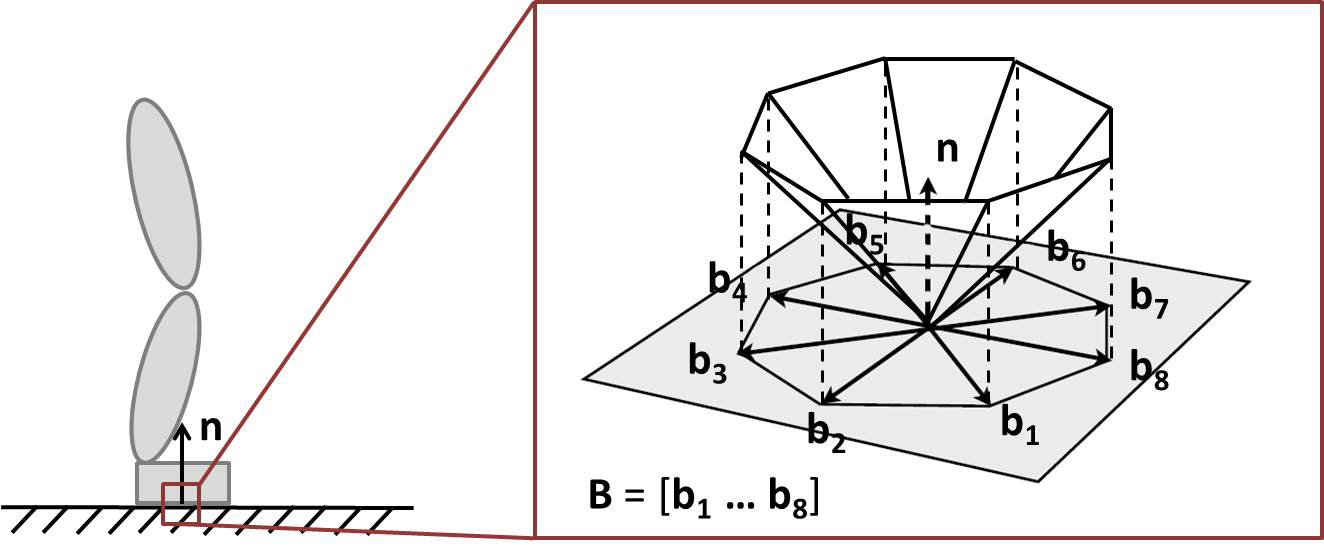
\includegraphics[width=0.85\textwidth]{figures/contact.jpg}
  \caption{A linearized friction cone used in LCP formulation. Left: a foot is in contact with the ground. Right, the friction cone at the contact point. $\vc{n}$ is the contact normal, and $\vc{b}_i$ are a set of tangential bases.}
  \label{fig:contactCone}
\end{figure}

Linear Complementarity Problem (LCP) is a more accurate and stable method to model contacts. The contact force $\vc{f}_c$ can be decomposed into the normal and the tangential (frictional) forces.
\begin{displaymath}
\vc{f}_c = f_\perp\vc{n}+\vc{B}\vc{f}_{\parallel}
\end{displaymath}
where $\vc{n}$ is the contact normal, $f_\perp$ and $\vc{f}_{\parallel}$ are the normal and tangential components respectively. $\vc{B}$ is a set of bases that span the tangential plane (Figure ~\ref{fig:contactCone}). The more basis $\vc{b}_i$ are used, the more accurate approximation of the friction cone is, but more computation is needed to solve the resulting LCP. 

LCP imposes a set of constraints to satisfy these three conditions of Columb friction: 1) In the normal direction, only repulsive forces are exerted to stop penetration. 2) In the tangential direction, the friction direction is opposite to the motion. 3) In the tangential direction, the friction can be either static or sliding. I will illustrate the concept of LCP using the formulation in the normal direction. The formulation in the tangential direction is beyond the scope of this chapter but can be found in these tutorials \cite{Lloyd:2005,Tan:2012b}. 

In a physical simulation, when two bodies collide, the relative velocity of the contact points can only be zero (resting) or positive (separating), but not negative (penetrating):
\begin{equation}
v_\perp\geq 0
\label{eq:separating}
\end{equation}
The normal contact force can be zero (no force) or positive (repulsive force) but not negative (sticking force):
\begin{equation}
f_\perp \geq 0
\label{eq:repulsive}
\end{equation}
The repulsive normal force only exists when the two bodies are in contact ($v_\perp\geq 0, f_\perp\geq 0$)
but not when they are separating ($v_\perp \geq 0, f_\perp =0$)
In other words, the following linear complementarity condition needs to be satisfied:
\begin{equation}
v_\perp f_\perp =0
\label{eq:complementarity}
\end{equation}

Combining the dynamics equations (eq. \ref{eq:dynamics} or ~\ref{eq:generalized}) and the LCP constraints (eq. \ref{eq:separating}, \ref{eq:repulsive}, \ref{eq:complementarity}) forms a mixed LCP problem, which can be solved efficiently by direct pivot-based methods \cite{Lloyd05} or iterative solvers \cite{Erleben:2007,Kaufman:2008,Otaduy:2009}. 


\subsection{Simulation Software}

There is a growing need for simulation software that can accurately simulate the complex dynamics of vitural humans and their interactions with their surrounding environment. A couple of open source physical simulators are readily available for research in physically-based character animation. The popular ones include Open Dynamic Engine (ODE) \cite{ode:2008}, Bullet \cite{bullet}, Dynamic Animation and Robotics Toolkit (DART) \cite{dart:2012} and MuJoCo \cite{mujoco}. All them can simulate articulated rigid body systems with LCP-based contact model in real time. These simulators allow the user to specify the structure of the articulated figure, the shape and the physical properties of each body, the type of joints, and other parameters describing the environment. Different simulators may offer different features, speed and accuracy. An in-depth comparison is beyond the scope of this Chapter. Erez et al.\cite{ErezTT15} provides an up-to-date review and comparison among these modern physical engines.
